\documentclass[10pt]{article}
\IfFileExists{neurips_2026.sty}{\usepackage[preprint]{neurips_2026}}{\usepackage[margin=1in]{geometry}}
\usepackage{amsmath,amssymb,amsthm,booktabs,graphicx,hyperref,microtype}
\usepackage[numbers]{natbib}
\newtheorem{theorem}{Theorem}
\newtheorem{proposition}{Proposition}
\title{Regime-Conditional Reward-Free Exploration}
\author{Anonymous Authors}\date{}
\begin{document}\maketitle
\begin{abstract}
We formulate reward-free exploration under hidden recurring transition
regimes. Training observes an unlabelled piecewise-stationary transition
stream; deployment supplies a short reward-free diagnostic phase in a
previously seen mode; only then is an arbitrary reward revealed. Our
Detect--Match--Explore (DME) construction quarantines boundaries, reuses
returning mode models, and diagnoses deployment before planning. We prove
conditional and diagnostic results but not the central detector segmentation
guarantee. A ten-seed tabular pilot finds a positive but practically small DME
advantage over restart, while a MiniGrid pilot favors pooling. Both
predeclared gates fail.
\end{abstract}

\section{Objective and relation to prior work}
Stationary RFE must support every post-hoc reward
\citep{jin2020rewardfree,kaufmann2021adaptive,zhang2021nearly}. DARLING studies
online reward-bearing non-stationary RL \citep{gerogiannis2026darling};
recurring-context work reuses reward-specific policies
\citep{alegre2021minimum}; latent MDPs optimize a known reward objective
\citep{kwon2021latent}; and active detection assumes known candidate models
\citep{duan2021detection}. Our distinct objective jointly requires learning
reward-uniform models from an unsegmented recurring stream and a
reward-independent deployment diagnostic.

Let unknown episodic kernels $\{P^{(m)}\}_{m=1}^M$ share finite state/action
spaces and horizon $H$. Hidden mode $z_k$ is fixed within each training episode,
switches only between episodes, may recur, and obeys a minimum dwell condition.
No training rewards, boundaries, or labels are observed. At deployment, a
previously learned mode $Z$ stays fixed for $q$ reward-free diagnostic episodes.
Then an arbitrary pathwise-unit-bounded reward $r$ is revealed and no further
interaction is allowed. The PAC objective is
\[
\Pr\!\left\{\sup_r[V^\star_{P^{(Z)}}(r)-
V^{\widehat\pi_r}_{P^{(Z)}}(r)]\le\epsilon\right\}\ge1-\delta .
\]

\section{Detect--Match--Explore}
DME executes reward-free probes, detects a transition change, quarantines an
uncertain boundary, and compares a confirmed segment with stored transition
models. A separated match resumes an existing mode-specific RFE learner;
otherwise DME creates a new entry. Deployment uses only a reward-free
transition prefix to match or reject before the reward is known. Assumptions
cover probe reachability, controlled transcript separation, clean occupancy,
dwell time, transition-only changes, and adaptively valid confidence sets.

\section{Established theory}
Let $\mathsf{SEG}$ mean that accepted samples are assigned to their correct
mode up to permutation, returning modes are matched, and quarantined samples
never contaminate an RFE learner.
\begin{theorem}
If $\mathsf{SEG}$ fails with probability $\delta_{\rm seg}$, each of $M$
stationary RFE calls has uniform error $\eta$ and failure
$\delta_{\rm rfe}$, and deployment diagnosis fails with probability
$\delta_{\rm id}$, then DME has uniform error $\eta$ with probability at least
$1-\delta_{\rm seg}-M\delta_{\rm rfe}-\delta_{\rm id}$.
\end{theorem}
\paragraph{Proof.} Intersect the stated success events and union bound.
\hfill$\square$
\begin{proposition}
For known models and fixed diagnostic strategy $\sigma$, maximum likelihood
obeys $\Pr_m(\widehat m\ne m)\le\sum_{\ell\ne m}
\operatorname{Aff}(\mathbb P_m^\sigma,\mathbb P_\ell^\sigma)$.
\end{proposition}
\begin{theorem}
With zero deployment observations, two exactly known modes can force
worst-case loss at least $1/2$.
\end{theorem}
\paragraph{Proof.} Reverse the good successors of two initial actions between
the modes; choosing one action with probability $p$ yields losses $p$ and
$1-p$. \hfill$\square$
\begin{theorem}
For two modes and any diagnostic test,
\[
\Pr_m(\psi=\ell)+\Pr_\ell(\psi=m)\ge
\tfrac12e^{-D_{\rm KL}(\mathbb P_m^\sigma\Vert\mathbb P_\ell^\sigma)} .
\]
\end{theorem}
This follows from binary testing and Bretagnolle--Huber
\citep{bretagnolle1978estimation}. A proof that the implemented detector
establishes $\mathsf{SEG}$ and an adaptive $M$-mode direct-sum RFE lower bound
remain open; neither is claimed.

\section{Measured pilots}
The finite-horizon tabular study uses ten seeds, two/three recurring modes, two
separations, and post-hoc target/adversarial rewards. Values are in $[0,1]$.
\begin{table}[h]\centering\caption{Tabular pilot; lower gap is better.}
\begin{tabular}{lrrr}
\toprule
Method & Units & Accept rate & Mean worst-reward gap \\
\midrule
Pooled & 40 & 1.000000 & 0.134720962030 \\
Restart, no reuse & 40 & 1.000000 & 0.002482741316 \\
Cluster, no quarantine & 40 & 1.000000 & 0.001268908213 \\
Recurrence-aware & 40 & 1.000000 & 0.001378200021 \\
Oracle boundary & 40 & 1.000000 & 0.001627412643 \\
Oracle mode & 40 & 1.000000 & 0.001566496241 \\
Sliding window & 40 & 1.000000 & 0.154578714875 \\
\bottomrule
\end{tabular}
\end{table}
DME's paired improvement over restart is 0.00110 with 95\% seed-bootstrap
interval $[0.00057,0.00178]$, below the predeclared 0.01 margin. Mean
recurrence saving is 48.1 transitions. The gate fails.
\begin{figure}[h]\centering
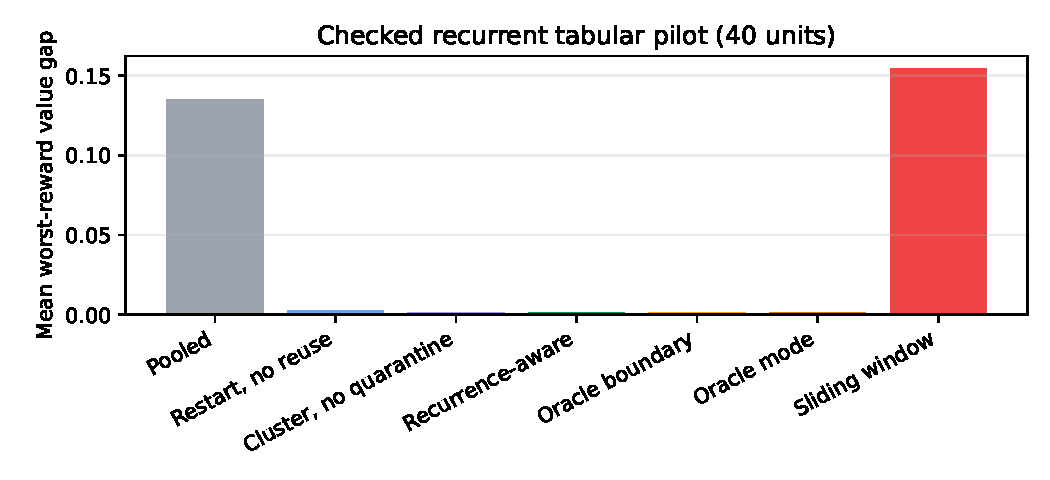
\includegraphics[width=.85\linewidth]{generated/figures/pilot_value_gaps.pdf}
\caption{Tabular worst-reward gaps generated from raw results.}\end{figure}

The ten-seed symbolic MiniGrid pilot also fails: DME beats restart (0.0492
versus 0.2648 worst-task gap) but pooling obtains zero gap; deployment-ID error
is 0.20.
\begin{table}[h]\centering\caption{MiniGrid pilot.}
\begin{tabular}{lrr}
\toprule
Method & Seeds & Mean worst-task gap \\
\midrule
pooled & 10 & 0.000000 \\
restart & 10 & 0.264844 \\
recurrence\_aware & 10 & 0.049219 \\
oracle\_upper\_bound & 10 & 0.000000 \\
\bottomrule
\end{tabular}
\end{table}

\section{Limitations and conclusion}
The key segmentation theorem is open, the base collector is not a faithful
named minimax RFE implementation, empirical reward families are finite, and
MiniGrid is too easy for pooling. Misdiagnosis can select an unsafe policy, so
abstention is necessary. Regime-conditional RFE is a distinct and testable
objective, but current theory and both failed gates preclude a NeurIPS-readiness
claim.

\bibliographystyle{plainnat}\bibliography{regime_rfe_references}
\end{document}
